\documentclass[svgnames]{beamer}

\usepackage[utf8]{inputenc}
\usepackage[T1]{fontenc}
\usepackage[french]{babel}
\usepackage{float}
\usetheme{Frankfurt}
\usepackage{enumitem}
\usepackage{pifont}
\usepackage{xcolor}
\usepackage{graphicx}
\usepackage{relsize}
\usepackage{array}
\usepackage{multirow}
\usepackage{multicol}
\usepackage{pgf, tikz}
\usetikzlibrary{arrows,shapes,positioning}
\usepackage{adjustbox}
\usepackage{makecell}
\usepackage[style=authoryear]{biblatex}

\def\checkmark{\tikz\fill[scale=0.4](0,.35) -- (.25,0) -- (1,.7) -- (.25,.15) -- cycle;}

\newenvironment{subitemize}{%
    \smaller
    \itemize
}{%
    \enditemize
}


%\setbeamertemplate{navigation symbols}{%
%	\insertframenumber/\inserttotalframenumber
%}
%
%\setbeamertemplate{headline}{%
%\leavevmode%
%  \hbox{%
%    \begin{beamercolorbox}[wd=\paperwidth,ht=2.5ex,dp=1.125ex]{palette quaternary}%
%    \insertsectionnavigationhorizontal{\paperwidth}{}{\hskip0pt plus1filll}
%    \insertsubsectionnavigationhorizontal{\paperwidth}{}{\hskip0pt plus1filll}
%    \end{beamercolorbox}%
%  }
%
%}

\definecolor{myblue}{cmyk}{1,.72,0,.38}
\definecolor{myblue2}{cmyk}{1,.65,0,.28}

\setbeamertemplate{bibliography item}{\insertbiblabel}

\newcommand{\mycite}[1]{[\textit{\cite{#1}}]}

\AtBeginSection[]
{
  \begin{frame}
  \frametitle{Plan}
  %\begin{multicols}{2}
  \tableofcontents[currentsection]
  %\end{multicols}
  \end{frame}
}

\addbibresource{biblio.bib}



\title[]{Contribution à l'apprentissage humain de gestes à l'aide de techniques de clustering pour l’analyse de mouvements capturés}
\author{Quentin Couland}
\institute{}
\date{\today}

\setbeamerfont{subsection in toc}{size=\small}
\setbeamerfont{subsection in toc}{size=\smaller}


\begin{document}

	\maketitle

	\part{Cadre}
	\section{Cadre de la thèse}
	\begin{frame}{\subsecname}
	\centering
		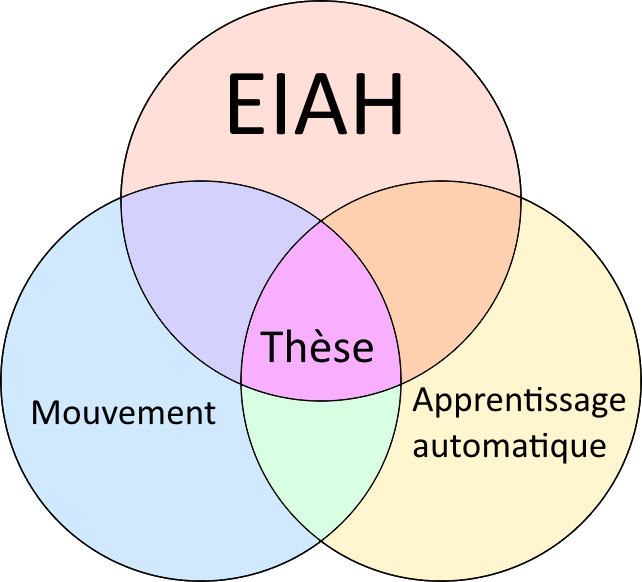
\includegraphics[scale=0.5]{img/venn_cadre.png}
	\end{frame}

	\subsection{EIAH}
	\begin{frame}{\subsecname}
	    \begin{block}{\mycite{Tchounikine2009PdR}}
	    « Environnements ayant pour but de favoriser l'apprentissage, en aidant, guidant et évaluant les apprenants d'une part et en assistant les enseignants d'autre part : que ce soit en présentiel, à distance, ou en situation mixte. »
	    \end{block}

	    \vspace{0.5cm}

	    Domaines d'utilisation multiples, mais un point en commun : la \textbf{pédagogie}.
	\end{frame}

	\subsection{Mouvement}
	\begin{frame}{Définition du mouvement}
	\begin{block}{Mouvement}
	Succession de postures dans le temps, espacées selon un pas de temps fixe ou variable.
	\end{block}
	\vspace{1cm}
	\centering
		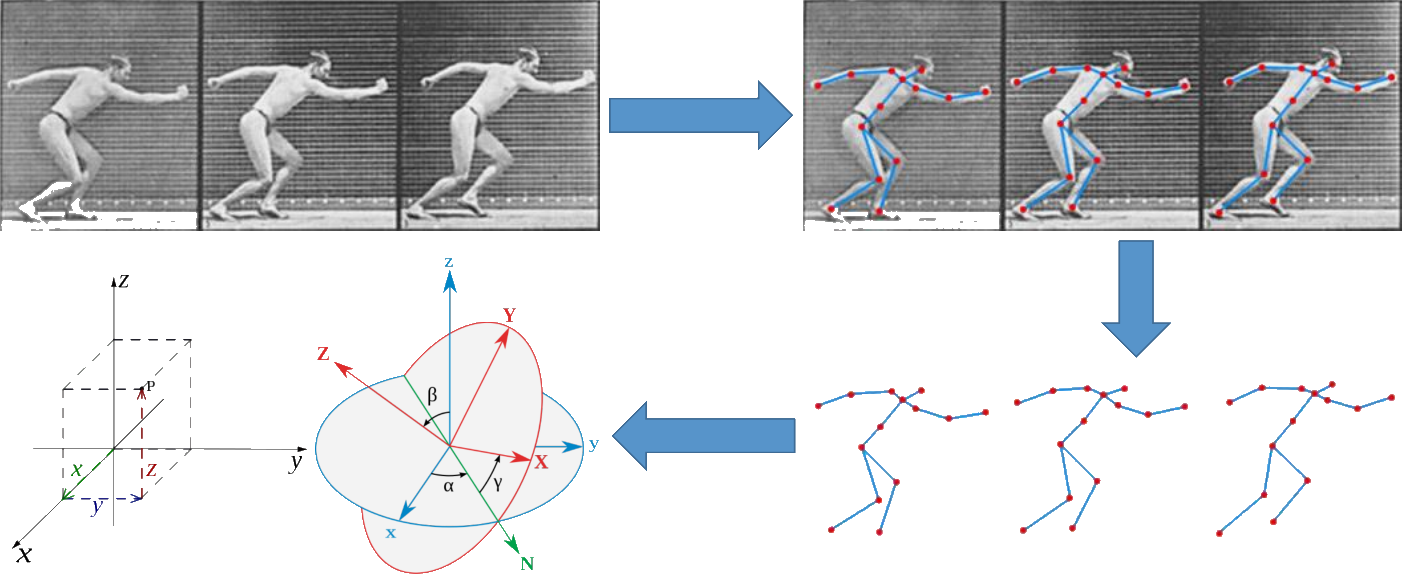
\includegraphics[scale=0.35]{img/mouvement_cadre.png}
	\end{frame}

	\subsection{Apprentissage automatique}
	\begin{frame}{\subsecname}
		Plusieurs familles d'algorithmes d'apprentissage automatique :
		\begin{block}{Apprentissage supervisé}
			\begin{itemize}[label=$-$]
				\item Classe les données à l'aide d'une fonction de séparation
				\item Apprentissage à l'aide d'une base de données annotées
			\end{itemize}
		\end{block}
		
		\begin{block}{Apprentissage non-supervisé}
			\begin{itemize}[label=$-$]
				\item Découverte de structure au sein de données
				\item Regroupement de données sans sémantique sur les groupes obtenus
				\item Évaluation de la forme des groupes obtenus
			\end{itemize}
		\end{block}
	\end{frame}
	
	\begin{frame}{\subsecname}
		\begin{block}{Apprentissage semi-supervise}
			\begin{itemize}[label=$-$]
				\item Apprentissage non-supervisé avec un petit nombre de données annotées
				\item Permet de donner une sémantique aux groupes obtenus
			\end{itemize}
		\end{block}
	\end{frame}
	
	\subsection{EIAH pour le mouvement}
	\begin{frame}{\subsecname}
		Plusieurs méthodes et objectifs pour les EIAH dédiés au mouvement :
		\begin{itemize}[label=$\bullet$]
			\item Affichage du mouvement à reproduire \mycite{Kora20151559}
			\item Manipulation d'objets \mycite{Chellali2016Aia}
			\item Immersion en réalité virtuelle (EVAH) \mycite{Baldominos2015AAt}
			\item Ludification \mycite{Alankus2010TCG}
		\end{itemize}

		\vspace{1cm}
	\end{frame}
	
	 \begin{frame}{Analyse des mouvements}
	 	Les données doivent être analysées, soit par un expert, soit par le système

		\begin{block}{Analyse empirique}
			Pas de formalisation des caractéristiques du geste, différences morphologiques, expertise difficile à formaliser (domaine médical)
		\end{block}
		
		\begin{block}{Analyse automatique}
			Connaissance experte formalisable et quantifiable
		\end{block}
	 \end{frame}

	
	\subsection{Limites des systèmes existants}
	\begin{frame}{\subsecname}
		Les EIAH dédiés à l'apprentissage du mouvement présentent souvent une ou plusieurs limites :
		\begin{block}{Limites généralistes}
			\begin{itemize}[label=$\bullet$]
				\item Conception \textit{ad-hoc}
				\item Intégration de la connaissance experte difficile sans ré-ingénierie conséquente
			\end{itemize}
		\end{block}
		
		\begin{block}{Limites de l'analyse automatique}
			\begin{itemize}[label=$\bullet$]
				\item Problème de la taille du corpus d'apprentissage
				\item Reconstitution d'un autre corpus pour un autre domaine applicatif
				\item Expert écarté du processus d'apprentissage
			\end{itemize}
		\end{block}
	\end{frame}
	
	\section{Problématiques de la thèse}
	\begin{frame}{\subsecname}
		\begin{itemize}[label=$-$]
			\item \textbf{Q1} : Comment développer un système permettant de caractériser le geste à l'aide de l'intégration de l'expertise d'un enseignant?
			\item \textbf{Q2} : Comment évaluer et comparer le geste (ou ses propriétés) de l'apprenant avec celui de l'enseignant afin d'évaluer la progression de l'apprentissage?
			\item \textbf{Q3} : Comment, dans une situation d'apprentissage de gestes donnée, proposer des retours pertinents et compréhensibles aux acteurs de l'apprentissage non spécialistes en analyse du mouvement?
		\end{itemize}
	\end{frame}

	\part{Etat de l'art}
	\section{Matériels de capture}
	\begin{frame}{Représentation informatique du mouvement}
		\centering
		\resizebox{!}{4cm}{%
		\begin{tikzpicture}
			\node[draw, rounded corners=3pt, align=center] (chest) at (0,-1.5) {chest};
			\node[draw, rounded corners=3pt, align=center] (neck) at (0,0) {neck};
			\node[draw, rounded corners=3pt, align=center] (head) at (0,1) {head};
			\node[draw, rounded corners=3pt, align=center] (leftshoulder) at (-2,0) {l. shoulder};
			\node[draw, rounded corners=3pt, align=center] (rightshoulder) at (2,0) {r. shoulder};
			\node[draw, rounded corners=3pt, align=center] (lefthand) at (-2,-1) {l. hand};
			\node[draw, rounded corners=3pt, align=center] (righthand) at (2,-1) {r. hand};
			\node[draw, rounded corners=3pt, align=center] (hips) at (0,-3) {hips (ROOT)};
			\node[draw, rounded corners=3pt, align=center] (leftknee) at (-2,-4) {l. knee};
			\node[draw, rounded corners=3pt, align=center] (rightknee) at (2,-4) {r. knee};
			\node[draw, rounded corners=3pt, align=center] (leftfoot) at (-2,-5) {l. foot};
			\node[draw, rounded corners=3pt, align=center] (rightfoot) at (2,-5) {r. foot};

			\node[] (hips_offset) at (-4,-3) {

			$\begin{array}{ccc}
                x & y & z \\
               (0 & 0 & 0) \\
            \end{array}$

			};


			\node[] (chest_offset) at (-4,-1.5) {

			$\begin{array}{ccc}
                x & y & z \\
               (0 & 1 & 0) \\
            \end{array}$

			};

			\node[draw] (c_base) at (-7,-2) {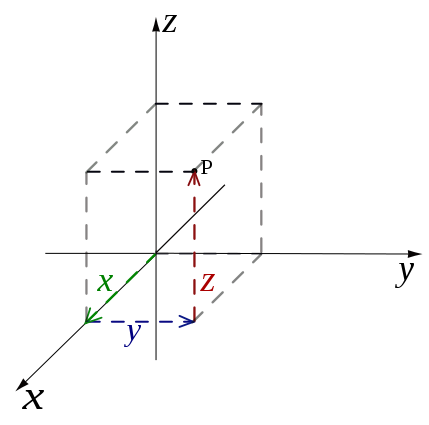
\includegraphics[scale=0.2]{img/coordinates.png}};



			\node[] (hips_orientation) at (4,-3) {

			$\begin{array}{ccc}
                \alpha & \beta & \gamma \\
               	(45 & 0 & 45) \\
            \end{array}$

			};


			\node[] (chest_orientation) at (4,-1.5) {

			$\begin{array}{ccc}
            	\alpha & \beta & \gamma \\
               	(78 & 10 & 21) \\
            \end{array}$

			};

			\node[draw] (c_base) at (-7,-2) {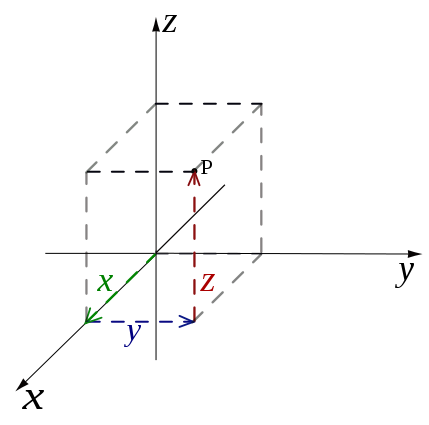
\includegraphics[scale=0.2]{img/coordinates.png}};

			\node[draw] (c_base) at (7,-2) {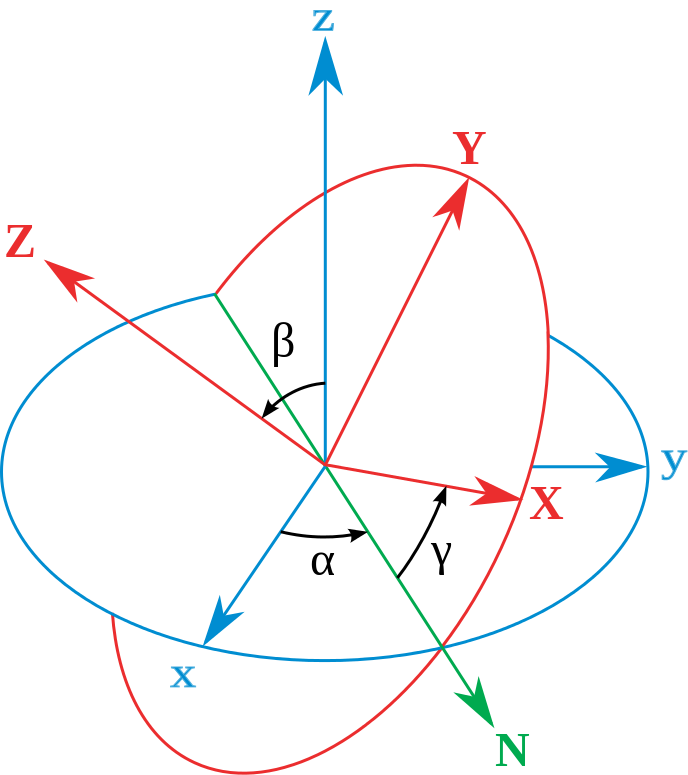
\includegraphics[scale=0.1]{img/euler_angles.png}};


			\draw(hips) -- (chest);
			\draw(chest) -- (neck);
			\draw(neck) -- (head);
			\draw(neck) -- (leftshoulder);
			\draw(leftshoulder) -- (lefthand);
			\draw(neck) -- (rightshoulder);
			\draw(rightshoulder) -- (righthand);
			\draw(hips) -- (leftknee);
			\draw(leftknee) -- (leftfoot);
			\draw(hips) -- (rightknee);
			\draw(rightknee) -- (rightfoot);

			\draw[loosely dotted, ->] (hips) -- (hips_offset);
			\draw[loosely dotted, ->] (chest) -- (chest_offset);

			\draw[loosely dotted, ->] (hips) -- (hips_orientation);
			\draw[loosely dotted, ->] (chest) -- (chest_orientation);
		\end{tikzpicture}
		}
	\end{frame}
	
	\subsection{Objectifs et coûts}
	\begin{frame}{Dispositifs de captation}
		Plusieurs objectifs possibles pour l'apprentissage du geste :
		\begin{itemize}[label=$\bullet$]
			\item Le mouvement est la finalité de l'apprentissage
			\item La manipulation d'un objet est la finalité de l'apprentissage 
		\end{itemize}
		
		Les dispositifs de captures ne sont pas les mêmes en fonction des objectifs et des contraintes :
		\begin{itemize}[label=$\bullet$]
			\item Objet de la captation
			\item Coût
			\item Qualité des données
			\item Encombrement
			\item Espace disponible
			\item Chaîne de traitement des données nécessaire
			\item Retours sensoriels ou visuels souhaités
		\end{itemize}
	\end{frame}
	
	\subsection{Caméra RGB}
	\begin{frame}{\subsecname}
		\begin{block}{Caméra RGB}
			\begin{itemize}[label=$\bullet$]
				\item Captation d'une vidéo
				\item Détermination d'un squelette à partir de la vidéo
			\end{itemize}
			Plusieurs méthodes d'extraction possible \mycite{Sarafianos2016DHp} : projection d'un squelette 3D en 2D pour obtenir une correspondance, utilisation de contraintes rigides sur plusieurs images successives, etc.\\
			Possibilité d'utiliser une vidéo stéréo pour reconstituer le squelette 3D \mycite{Liu2016Tb3}
		\end{block}
	\end{frame}
	
	\subsection{Caméra RGB-D}
	\begin{frame}{\subsecname}
		\begin{block}{Caméra RGB-D}
			\begin{itemize}[label=$\bullet$]
				\item Captation d'une vidéo + une carte de profondeur
				\item Pas d'inférence à partir d'une image 2D seulement
				\item Problème d'occlusion (possibilité d'utiliser plusieurs caméras synchronisées \mycite{Regazzoni2014Rcv}, mais nécessite un emplacement de capture dédié)
			\end{itemize}
			Sport \mycite{YAMAOKA2013912, Yoshinaga2015Doa, Kora20151559}, 
		\end{block}
	
	\end{frame}
	
	\subsection{Caméras infrarouge}
	\begin{frame}{\subsecname}
		\begin{block}{Caméras infrarouge}
			\begin{itemize}[label=$\bullet$]
				\item Meilleur précision
				\item Plusieurs captures possibles en simultané \mycite{Pfister2014Cao, Yang2016HUL}
				\item Coût très élevé
				\item Nécessite un environnement de capture dédié
				\item Chaîne de traitement lourde
			\end{itemize}
		\end{block}
	\end{frame}
	
	\subsection{Capteurs inertiels portables}
	\begin{frame}{\subsecname}
		\begin{block}{Capteurs inertiels portables}
			\begin{itemize}[label=$\bullet$]
				\item Ensemble de capteurs généralement reliés entre eux
				\item Transmission sans fil possible \mycite{PORCIUNCULA2018S220}
				\item Constitués d'un ou d'une combinaison des dispositifs suivants : accéléromètre, gyromètre et magnétomètre
				\item Utilisation dans des environnements variés
				\item Qualité des données variables (perturbations de l'environnement, qualité de la liaison avec l'ordinateur recevant les données, etc.)
				\item Chaîne de traitement à utiliser pour améliorer les données \mycite{Roetenberg2005Com}
				\item Également utilisés dans certains casques de réalité virtuelle \mycite{HTCViveSpecs}
			\end{itemize}
		\end{block}
	\end{frame}
	
	\subsection{Captation pour la manipulation d'objets}
	\begin{frame}{\subsecname}
		\begin{block}{Interfaces haptiques}
			\begin{itemize}[label=$\bullet$]
				\item Permettent la manipulation d'un objet virtuel
				\item Retours sensitif possible (retour de force, tactile, etc.)
				\item Utilisation possible avec des environnements virtuels, afin de favoriser l'immersion \mycite{Whitmire2018}
				\item Très utilisés dans le cadre de l'apprentissage de manipulation d'objets médicaux \mycite{CORREA20196, Choi2015103, PEPLEY20171066, HALABI20189}
				\item Utilisation dans le cadre de l'industrie, pour simuler la manipulation d'objets \mycite{Chamaret2010}
			\end{itemize}
		\end{block}
	\end{frame}
	
	\section{EIAH pour l'apprentissage du geste}
	\begin{frame}{\secname}
		De nombreux EIAH aux finalités différentes :
		\begin{itemize}[label=$\bullet$]
			\item Apprentissage actif impliquant l'étudiant \mycite{Xu2019Ptt}
			\item Rééducation \mycite{Alankus2010TCG}
			\item Amélioration de la performance sportive \mycite{Baldominos2015AAt}
			\item etc.
		\end{itemize}
		
		Mais également dans des domaines variés :
		\begin{itemize}[label=$\bullet$]
			\item Médical (analyse de postures \mycite{Aminian2004Chm}, chirurgie \mycite{BMT_2015}, etc.)
			\item Sport (danse \mycite{Maes2012DtM}, archerie japonaise \mycite{Yoshinaga2015Doa}, lancer de disques \mycite{YAMAOKA2013912}, etc.)
		\end{itemize}
	\end{frame}
	
	\begin{frame}{\secname}
		Baldominos \textit{et al.} : Mise en situation dans un environnement virtuel, intervention de l'expert pour régler les paramètres des exercices (intensité, parties du corps qui travaillent, etc.) \mycite{Baldominos2015AAt}\\
		\centering
		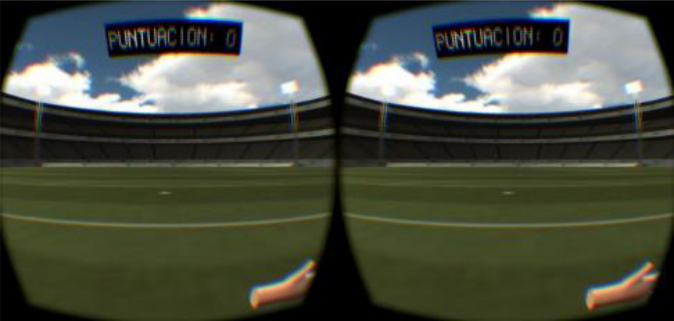
\includegraphics[scale=0.5]{img/eiah_baldominos.png}
	\end{frame}
	
	\begin{frame}{\secname}
		Toussaint : Manipulation d'un trocard, en combinant les données d'un bras haptique et du retour de force associé et d'un occulomètre (pour suivre la trajectoire du regard). \mycite{BMT_2015}\\
		\centering
		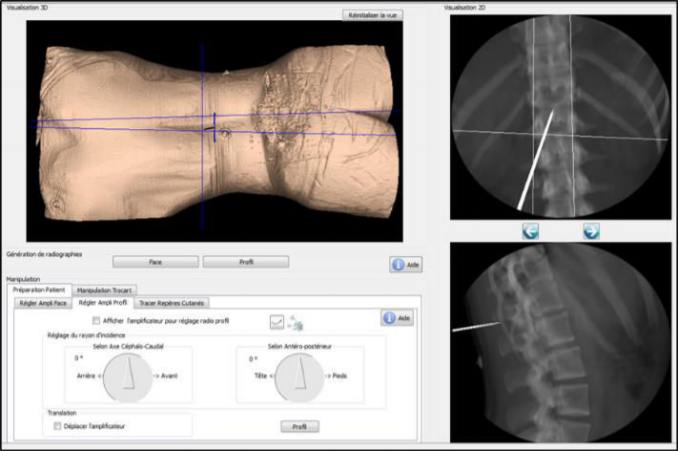
\includegraphics[scale=0.4]{img/eiah_toussaint.png}
	\end{frame}
	
	\begin{frame}{\secname}
		 Gameiro \textit{et al.} : Ludification de l'apprentissage de la langue des signes \mycite{Gameiro2014KST}\\
		\centering
		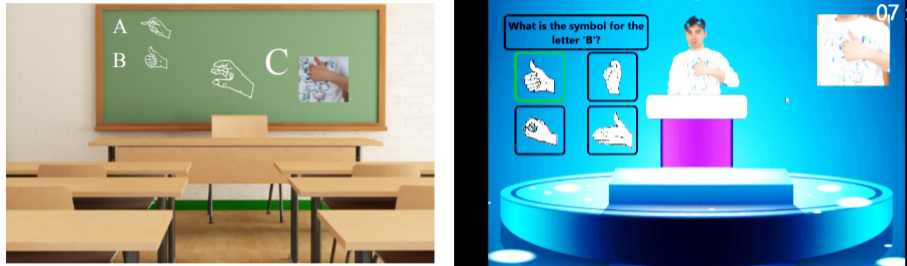
\includegraphics[scale=0.4]{img/eiah_gameiro.png}
	\end{frame}
	
	\begin{frame}{\secname}
		 Xu \textit{et al.} : Apprentissages de gestes variés (manipuler un métier à tisser, tirer à l’arc, chevaucher un cheval, manipuler des panneaux) à l'aide de l'adaptation du parcours d'apprentissage \mycite{Xu2019Ptt}\\
		\centering
		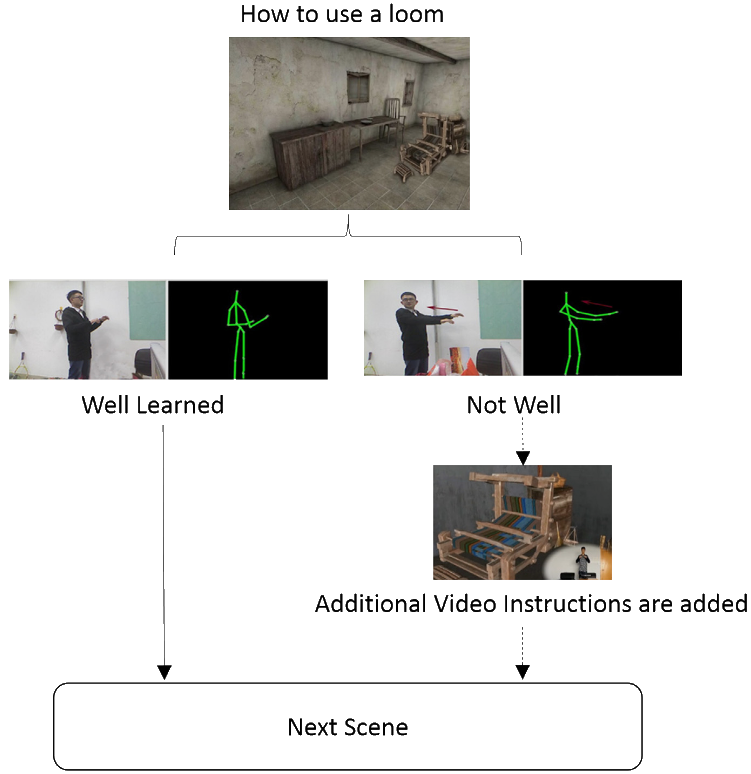
\includegraphics[scale=0.3]{img/eiah_xu.png}
	\end{frame}
	
	\begin{frame}{\secname}
		 Morel : évaluation de gestes sportifs à l'aide de séries temporelles. Les mouvements de l'apprenant et de l'expert sont recalés spatialement et temporellement, puis les erreurs sont calculés et affichées \mycite{Morel2017Mts}\\
		\centering
		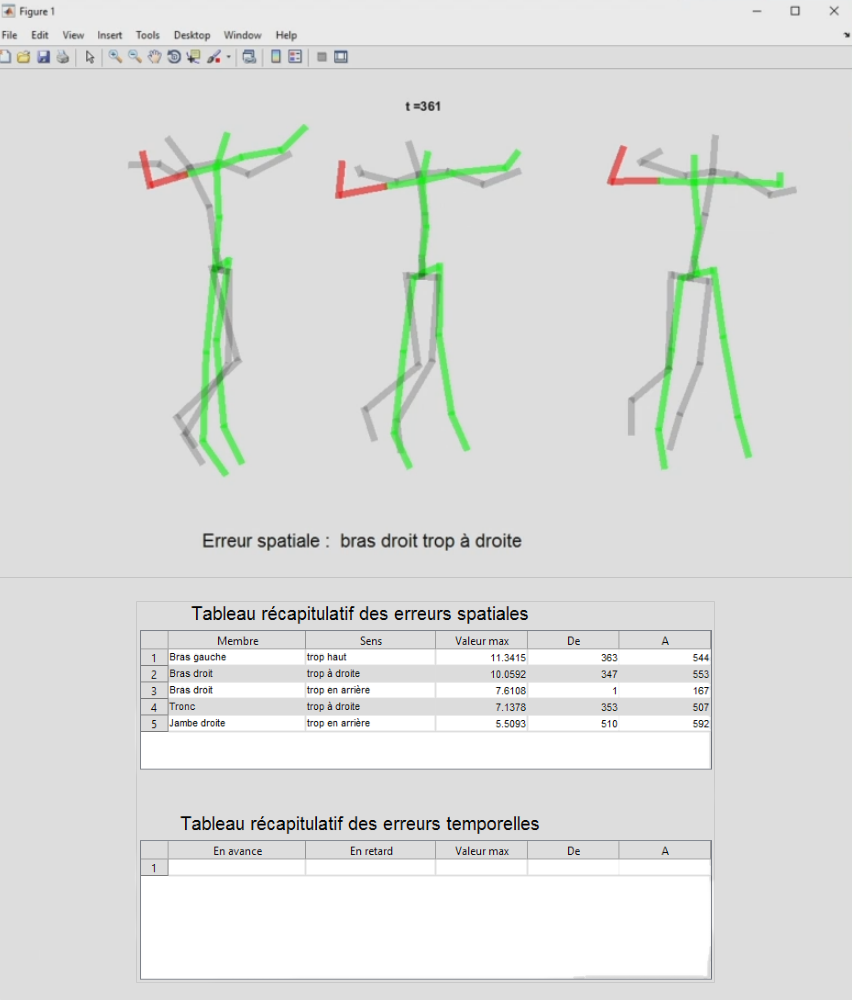
\includegraphics[scale=0.25]{img/eiah_morel.png}
	\end{frame}
	
	\begin{frame}{\secname}
		Plusieurs limites récurrentes :
		\begin{itemize}[label=$\bullet$]
			\item Ré-ingénierie nécessaire pour utiliser l'EIAH dans d'autres domaines
			\item Dans le cas d'apprentissage supervisé, nécessite une base de donnée d'apprentissage étiquetée conséquente, la reconstitution d'un corps pour l'utilisation dans un autre domaine et la connaissance précise des classes \textit{a priori}
			\item Dans les systèmes automatiques (s'affranchissant de l'expert), les retours peuvent manquer de sémantique, et les retours peuvent être difficile à interpréter pour des non-experts
		\end{itemize}
	\end{frame}
	
	\section{Descripteurs du mouvement}
	\begin{frame}{Représentation informatique du mouvement}
		\begin{center}Position et orientation\end{center}
        \begin{table}
			\begin{adjustbox}{max width=\textwidth}
				\begin{tabular}{c|cccccc}
        		& \multicolumn{2}{c}{articulation 1}  & \multicolumn{2}{c}{articulation 2} & \multicolumn{2}{c}{articulation 3}\\\hline
        		frame 1 & [(0,0,0) & (45,0,45)]     & [(0,1,0)  & (78,10,21)]   & [(0,1,0) & (12,53,120)]\\
        		frame 2 & [(5,4,7) & (42,1.1,45.2)] & [(0,2,0)  & (74,8,32)]    & [(1,3,4) & (11,54,121)]\\
        		frame 3 & [(5,8,7) & (48,1.1,44.2)] & [(1,2,3)  & (75,8,38)]    & [(2,0,4) & (112,55,10)]\\
        		frame 4 & [(7,3,8) & (1,101,14.4)]  & [(17,3,10)  & (121,4,38)]    & [(8,3,1) & (121,254,17)]\\
        		frame 5 & [(5,8,7) & (48,1.1,44.2)] & [(1,2,3)  & (75,8,38)]    & [(2,0,4) & (112,55,10)]\\
        		frame 6 & [(5,4,7) & (42,1.1,45.2)] & [(0,2,0)  & (74,8,32)]    & [(1,3,4) & (11,54,121)]\\
        		frame 7 & [(7,3,8) & (1,101,14.4)]  & [(17,3,10)  & (121,4,38)]    & [(8,3,1) & (121,254,17)]\\
        		frame 8 & [(17,8,1) & (1,101,14.4)]  & [(1,3,8)  & (78,4,25)]    & [(2,1,1) & (45,78,157)]\\
        		frame 9 & [(11,0,0) & (1,14,18.4)]  & [(17,3,10)  & (121,4,38)]    & [(4,11,12) & (125,47,1)]\\
        		frame 10 & $\underbrace{[(3,4,2)}_\text{position}$ & $\underbrace{(46,1.3,47.2)]}_\text{orientation}$ & [(0,1,0) & (75,5,12)] & [(1,8,7) & (11,53,119)]\\
        		\end{tabular}
        	\end{adjustbox}
        \end{table}
	\end{frame}
	
	\begin{frame}{\secname}
		Nécessité d'observer certaines \textbf{caractéristiques} du mouvement, afin de pouvoir en extraire des \textbf{informations pertinentes} dans le contexte de l'analyse.
		
		\begin{block}{Descripteur du mouvement}
			Un descripteur est un indicateur calculé à partir du mouvement brut :  « Des observables signifiant sur le plan pédagogique » calculés à partir de traces (tous types de données, générées à partir des interactions de l’étudiant avec le système) ou d’autres indicateurs \mycite{Choquet2007MTf}
		\end{block}
	\end{frame}
	
	\subsection{Classifications des descripteurs}
	\begin{frame}{\subsecname}
		Plusieurs classifications de descripteurs existent :
		\begin{itemize}[label=$\bullet$]
			\item Laban Movement Analysis (LBA) :  annotation hiérarchique pour caractériser originellement les mouvements de danse. Quatre informations sont quantifiées : la direction, la durée, la partie du corps concernée et la dynamique du mouvement
			\item Aristidou \textit{et al.} : caractérisation de la danse folklorique à l'aide du système LBA \mycite{Aristidou2015FDE}
		\end{itemize}
		
		\centering
		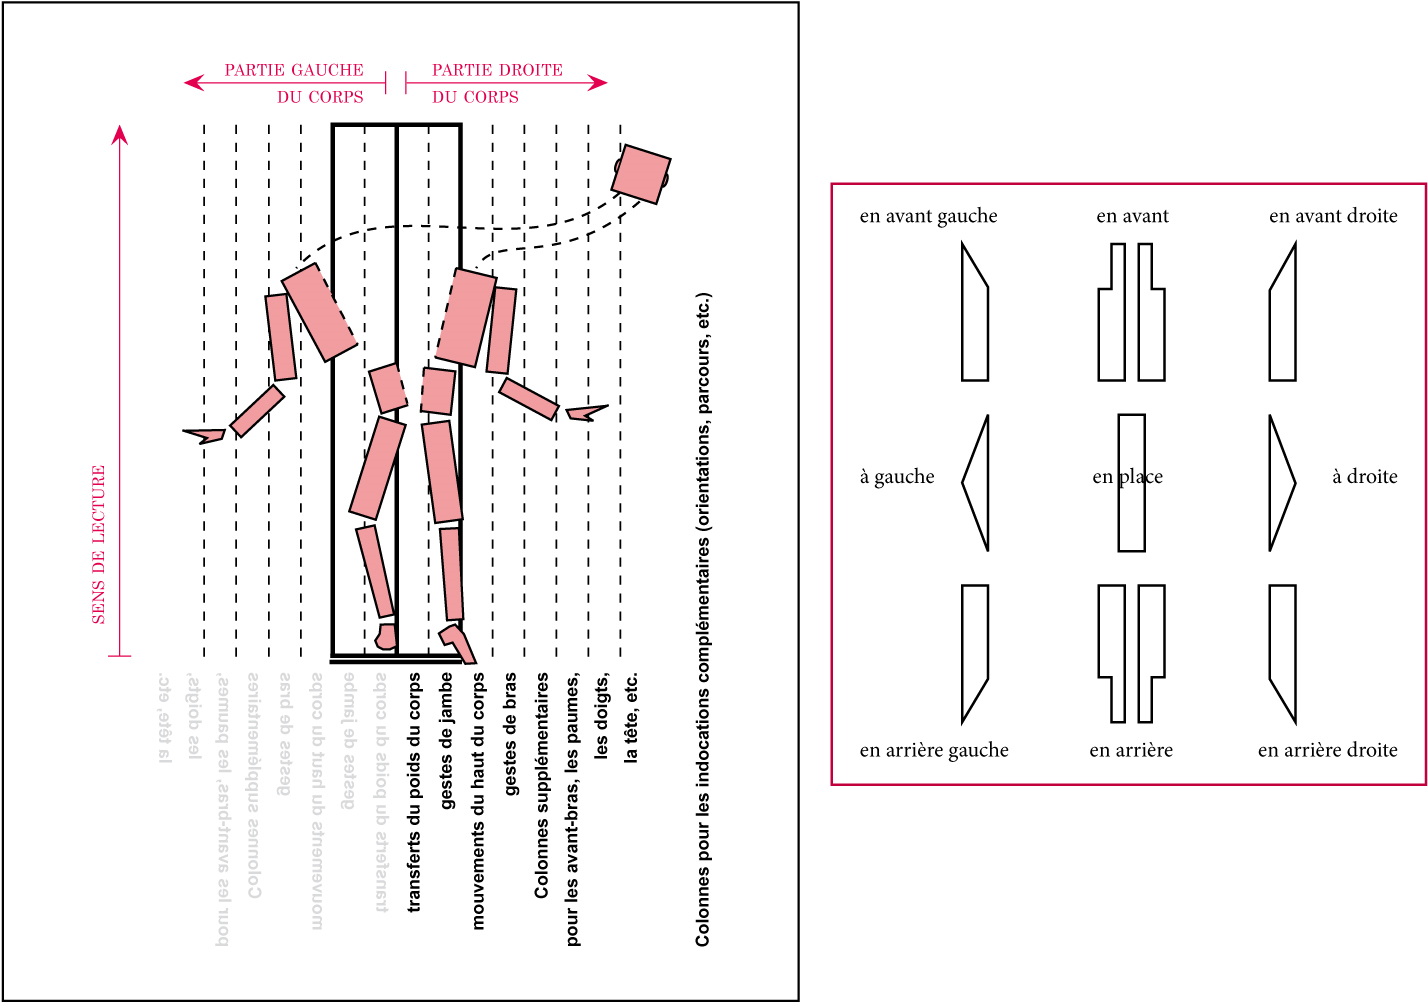
\includegraphics[scale=0.15]{img/laban_2.png}
	\end{frame}
	
	\begin{frame}{\subsecname}
		\begin{itemize}[label=$\bullet$]
			\item Larboulette et Gibet : classification en descripteurs bas-niveau (quantités cinématiques, dynamiques ou géométrique) / haut-niveau (quantités exploitables dans une évaluation visuelle du mouvement ou par un expert), cinématique / géométrique, corps / environnement \mycite{larboulette2015Descriptors}
			\item Morel : classification en trois grandes familles, descripteurs reposant sur un modèle du corps humain, holistiques (dynamique globale de l'objet considéré) et descripteurs locaux (à partir de points d'intérêt isolés) \mycite{Morel2017Mts}
		\end{itemize}
	\end{frame}
	
	\begin{frame}{\subsecname}
		Ensembles de descripteurs pour l'indexation et la recherche de mouvement :
		\begin{itemize}[label=$\bullet$]
			\item Sakurai \textit{et al.} : plusieurs aires extraites d'un pentagone calculé, puis utilisation de la DTW pour la recherche \mycite{Sakurai2015Ros}
			\item Xiao \textit{et al.} : projection du mouvement 3D sur 8 plans 2D, puis réduction à l'aide d'un algorithme de séléction de caractéristiques semi-supervisé \mycite{Xiao2015Sbh}
		\end{itemize}
	\end{frame}
	
	\begin{frame}{\subsecname}
		Ensembles de descripteurs pour la reconnaissance d'actions :
		\begin{itemize}[label=$\bullet$]
			\item  Delaye et Anquetil : descripteurs servant à caractériser les mouvements d'écriture : points de début et de fin de trait, angles formés par les différentes parties des lettres, proportion de trajectoires dirigées, etc. (HBF49) \mycite{Delaye2013HBF}
			\item Boulahia \textit{et al.} : généralisation de HBF49 à une trajectoire 3D (HIF3D) \mycite{Boulahia2016HIF}
			\item Rao \textit{et al.} : caractérise les moments d'inflexion dans la trajectoire, afin de les segmenter en unités élémentaires \mycite{Rao2002VRR}
		\end{itemize}
	\end{frame}
	
	\begin{frame}{\subsecname}
		\begin{itemize}[label=$\bullet$]
			\item Réutisabilité non assurée
			\item Utilisation dans un contexte d'apprentissage non considérée
			\item Compréhension et utilisation par un humain non assurées
			\item Redondance sémantique
		\end{itemize}
	\end{frame}
	
	\subsection{Classifications en descripteurs élémentaires}
	\begin{frame}{\subsecname}
	Proposition de classification en descripteurs élémentaires
		\begin{itemize}[label=$\bullet$]
			\item Descripteurs non issus de calculs, de ré-interprétations ou d'ensembles de descripteurs « bas-niveau » du mouvement
			\item Répondent à des besoins d'observation et d'analyse
		\end{itemize}
	\end{frame}
	
	\section{Analyse du mouvement capturé}
	\begin{frame}{\secname}
		Il existe plusieurs manières d'analyser le geste :
		\begin{itemize}[label=$\bullet$]
			\item Analyse par observation humaine
			\item Analyse par observation d'indicateurs
			\item Analyse par détection de séquence ordonnée d'actions
			\item Analyse basée sur des techniques d'apprentissage automatique
		\end{itemize}
	\end{frame}
	
	\subsection{Analyse par observation humaine}
	\begin{frame}{\subsecname}
		\begin{block}{Domaine médical}
			\begin{itemize}[label=$\bullet$]
				\item Rééducation
				\item Visualisation de la démarche du patient à distance (analyse de la démarche \mycite{Chen2016TPG})
				\item Entraînement de plusieurs chirurgiens dans un environnement virtuel (chirurgie \mycite{Pulijala2017VRS}), etc.
			\end{itemize}
		\end{block}
	\end{frame}
	
	\begin{frame}{\subsecname}
		\begin{block}{Sport}
			\begin{itemize}[label=$\bullet$]
				\item Analyse des vidéos de l'apprenant avant et après l'entrainement (visualisation puis reproduction du mouvement de l'expert en karaté, \mycite{Burns2011Uvh})
				\item Superposition du modèle de l'apprenant et de l'expert pour la reproduction et l'apprentissage (lancer au football américain, \mycite{LeNaour2019S3V})
				\item Projection du modèle de l'apprenant sur celui de l'expert en temps réel (golf, \mycite{Kora20151559})
				\item Superposition de l'apprenant à un ou des modèles experts, en fonction (archerie japonaise, \mycite{Yoshinaga2015Doa})
			\end{itemize}
		\end{block}
	\end{frame}
	
	\subsection{Analyse par observation d'indicateurs}
	\begin{frame}{\subsecname}
		\begin{block}{Domaine médical}
			\begin{itemize}[label=$\bullet$]
				\item Comparaison de la trajectoire d'un objet par rapport à une trajectoire de référence (forceps \mycite{Pham2010Tdg}, porte-aiguille \mycite{Despinoy2016UTS})
				\item Analyse de l'évolution de la maladie de Parkison, à l'aide de la distance réalisée à chaque pas, balancement de la posture, degré de balancement des bras et constance de l'intervalle de temps entre deux pas \mycite{Wang2013HMM}
			\end{itemize}
		\end{block}
	\end{frame}
	
	\begin{frame}{\subsecname}
		\begin{block}{Sport}
			\begin{itemize}[label=$\bullet$]
				\item Analyse basée sur les positions relatives des parties du corps à des moments clés du lancer (lancer de disque, \mycite{Yamaoka2013FoF})
				\item alignement spatial d'un membre par rapport au membre de référence, et différence entre les chemins de déformations induits par les alignements des membres de l’apprenant et de l’expert \mycite{Morel2017Mts}
				\item Trajectoire et vitesse du poignet (service au tennis, \mycite{Makio2007DoS})
			\end{itemize}
		\end{block}
	\end{frame}
	
	\begin{frame}{\subsecname}
		\begin{block}{Arts}
			\begin{itemize}[label=$\bullet$]
				\item Analyse de la correlation spatiale et temporelle entre le modèle de l'apprenant et de l'expert (danse \mycite{Maes2012DtM})			
				\item Décomposition du mouvement à l'aide d'un seul descripteur projeté dans un espace sphérique, puis comparaison à une base de données de mouvements de danse (danse \mycite{Kyan2015ABD})
				\item Détermination du mode jeu à l'aide d'informations cinétiques du mouvement : vitesse, tremblement, impulsion (violon \mycite{Rasamimanana2008EbA})
			\end{itemize}
		\end{block}
	\end{frame}
	
	\subsection{Analyse par détection de séquence ordonnée d'actions}
	\begin{frame}{\subsecname}
		\begin{block}{Environnements virtuels}
			\begin{itemize}[label=$\bullet$]
				\item Description du scénario pédagogique par l'expert, à l'aide d'une association activité / séquence d'actions, elles-mêmes divisées en séquences de comportement élémentaires : observation, déplacement, interaction, communication \mycite{Mahdi2019TaE}		
				\item Proposition d'un parcours à réaliser par l'expert, personnalisable à l'aide de points de contrôle à passer dans un ordre précis, puis détection de la présence d'un objet ou du corps de l'apprenant au sein de ces zones pour segmenter le mouvement. Enfin, chaque segment est comparé à la référence de l'expert \mycite{Delest2019MaE}
			\end{itemize}
		\end{block}
	\end{frame}
	
	\subsection{Analyse basée sur des techniques d'apprentissage automatique}
	\begin{frame}{\subsecname}
		\begin{block}{Analyse automatique}
			\begin{itemize}[label=$\bullet$]
				\item Évaluation de gestes sans \textit{a priori} sur le geste en lui-même, afin de déterminer les règles sous-jacentes à l'évaluation subjective des experts (patinage artistique et plongeon olympiques \mycite{Pirsiavash2014AQA})
				\item Segmentation, reconnaissance et évaluation de gestes à l'aide d'algorithmes de logique floue. Extraction de descripteurs cinétiques, reconnaissance à l'aide de classifieurs binaires pré-entrainés, puis évaluation par rapport aux mouvements contenus dans une base de données (gestes divers \mycite{Patrona2018MaA})
			\end{itemize}
		\end{block}
	\end{frame}
	
	\subsection{Bilan des systèmes existants}
	\begin{frame}{\subsecname}
		\begin{block}{Systèmes basés sur l'analyse humaine}
			\begin{itemize}[label=$\bullet$]
				\item Utilisateurs finaux au centre du système
				\item Savoir de l'expert parfois indispensable et non aisément formalisable (domaine médical)
				\item Parfois pas utilisables par un non-expert (nécessité de combiner les retours du système à une expertise scientifique)
				\item Possibilité de proposer des visualisations du mouvement de l'expert et de l'apprenant, facilement utilisables par un non-expert et génériques, mais ne proposent pas d'analyse
			\end{itemize}
		\end{block}
		
		\begin{block}{Systèmes utilisant des descripteurs}
			\begin{itemize}[label=$\bullet$]
				\item Fournissent un ensemble de valeur permettant d'assister l'expert dans son jugement
				\item Nécessiter de posséder des connaissances scientifiques pour l'interprétation des valeurs
				\item Souvent fortement couplés au domaine applicatif choisi, ainsi qu'au matériel utilisé
			\end{itemize}
		\end{block}
	\end{frame}
	
	\begin{frame}{\subsecname}
		\begin{block}{Systèmes d'analyse automatique}
			\begin{itemize}[label=$\bullet$]
				\item Permettent de s'affranchir de l'expert une fois le système conçu
				\item Retours parfois peu exhaustif (score seulement, sans indication sur les parties du corps qui ne font pas correctement le geste)
				\item Manque d'indications sur comment corriger le geste
				\item L'absence d'expert lors de l'utilisation limite l'exhaustivité des retours
				\item Généricité au regard du domaine considéré souvent faible
			\end{itemize}
		\end{block}
		
		\begin{block}{Systèmes basés sur la détection d'actions}
			\begin{itemize}[label=$\bullet$]
				\item Cherchent à segmenter le mouvement en unités élémentaires, puis proposent une comparaison de l'ordre de ces unités élémentaires
				\item Intégration de la connaissance experte dès la conception, manque de généricité
				\item Certains systèmes introduisent la réutilisabilité dès leur conception \mycite{Mahdi2019TaE, Delest2019MaE}
			\end{itemize}
		\end{block}
		
		\begin{block}{Systèmes basés sur l'apprentissage automatique}
			\begin{itemize}[label=$\bullet$]
				\item Intégration de la connaissance experte \textit{a priori}
				\item Nécessitent une base de données (d'apprentissage et de comparaison) volumineuse et spécialisée
			\end{itemize}
		\end{block}
	\end{frame}
	
	\subsection{Positionnement}
	\begin{frame}{\subsecname}
		\begin{itemize}[label=$\bullet$]
			\item Assistance à l'expert dans sa tâche d'analyse
			\item Système d'évaluation du geste, proposant également des indicateurs visuels pour l'expert
			\item Intégration de la connaissance experte avant l'utilisation en situation d'apprentissage, mais sans de ré-ingénierie nécessaire 
		\end{itemize}
	\end{frame}

	\part{Contributions}
	\section{Motion Learning Analytics}
	\begin{frame}{\secname}
		\begin{block}{Motion Learning Analytics (MLA)}
			\begin{itemize}[label=$\bullet$]
				\item Propose un ensemble d'outils pour pré-traiter et extraire des informations permettant d'analyser un geste
				\item Permet également de comparer les mouvements à ceux d'un expert, à l'aide de techniques de clustering
				\item Propose un ensemble de métriques, ainsi que de visualisation pour assister l'expert dans sa tâche d'évaluation des gestes
			\end{itemize}
		\end{block}
	\end{frame}
	
	\subsection{Architecture MLA}
	\begin{frame}{\subsecname}
	\centering
		\includegraphics[scale=0.3]{img/mla/MLA_color_1.png}
	\end{frame}

	\begin{frame}{\subsecname}
	\centering
		\includegraphics[scale=0.3]{img/mla/MLA_color_2.png}
	\end{frame}

	\begin{frame}{\subsecname}
	\centering
		\includegraphics[scale=0.3]{img/mla/MLA_color_3.png}
	\end{frame}

	\begin{frame}{\subsecname}
	\centering
		\includegraphics[scale=0.3]{img/mla/MLA_color_4.png}
	\end{frame}

	\begin{frame}{\subsecname}
	\centering
		\includegraphics[scale=0.3]{img/mla/MLA_color_5.png}
	\end{frame}

	\begin{frame}{\subsecname}
	\centering
		\includegraphics[scale=0.3]{img/mla/MLA_color_6.png}
	\end{frame}

	\begin{frame}{\subsecname}
	\centering
		\includegraphics[scale=0.3]{img/mla/MLA_color_7.png}
	\end{frame}

	\begin{frame}{\subsecname}
	\centering
		\includegraphics[scale=0.3]{img/mla/MLA_color_8.png}
	\end{frame}

	\begin{frame}{\subsecname}
	\centering
		\includegraphics[scale=0.3]{img/mla/MLA_color_9.png}
	\end{frame}

	\begin{frame}{\subsecname}
	\centering
		\includegraphics[scale=0.3]{img/mla/MLA_color_10.png}
	\end{frame}

	\begin{frame}{\subsecname}
	\centering
		\includegraphics[scale=0.3]{img/mla/MLA_color_11.png}
	\end{frame}

	\begin{frame}{\subsecname}
	\centering
		\includegraphics[scale=0.3]{img/mla/MLA_color_12.png}
	\end{frame}

	\begin{frame}{\subsecname}
	\centering
		\includegraphics[scale=0.3]{img/mla/MLA_color_13.png}
	\end{frame}

	\begin{frame}{\subsecname}
	\centering
		\includegraphics[scale=0.3]{img/mla/MLA_color_14.png}
	\end{frame}

	\begin{frame}{\subsecname}
	\centering
		\includegraphics[scale=0.3]{img/mla/MLA_color_15.png}
	\end{frame}

	\begin{frame}{\subsecname}
	\centering
		\includegraphics[scale=0.3]{img/mla/MLA_color_16.png}
	\end{frame}

	\subsection{Workflow du système MLA}
	\begin{frame}{\subsecname}
	\centering
		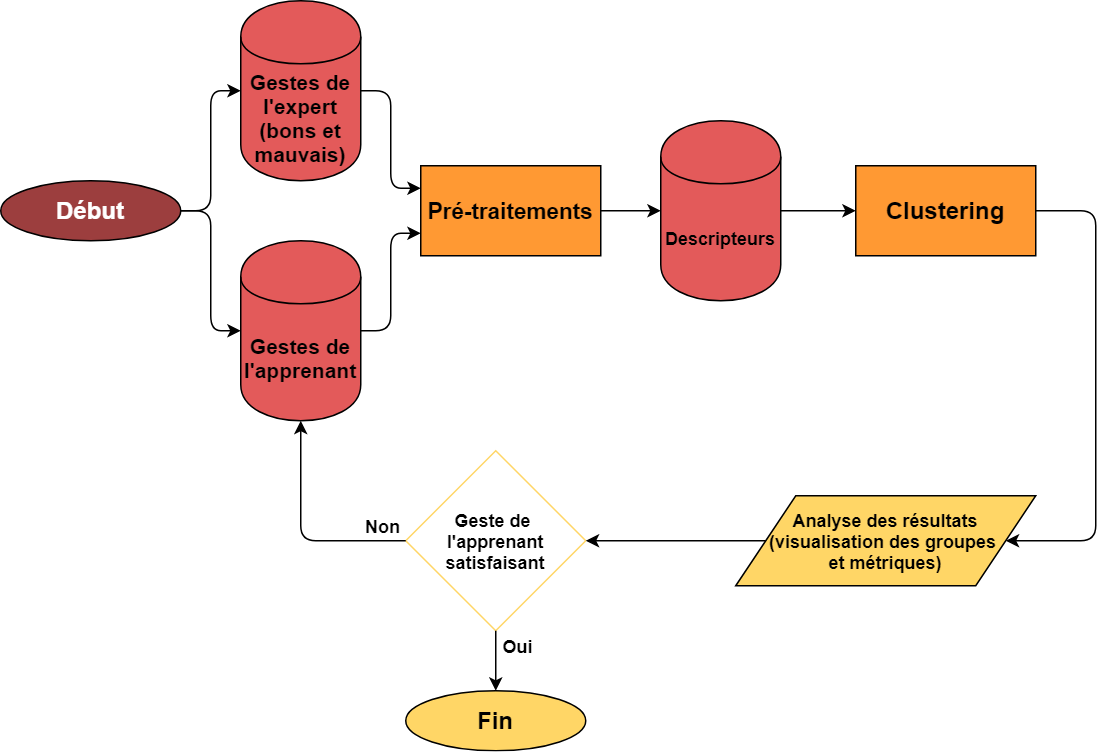
\includegraphics[scale=0.3]{img/workflow_MLA.png}
	\end{frame}

	\section{Traitements des données}
	
	\subsection{Matériel de capture}
	\begin{frame}{Perception Neuron}
		
	\end{frame}
	
	\subsection{Taille des membres}
	\begin{frame}{Variation de la taille des membres}
		Fixation de la taille des membres à l'aide de la posture de référence (posture à l'indice 0)
	\end{frame}
	
	\subsection{Incohérence des positions}
	\begin{frame}{Incohérence des positions successives}
	\centering
		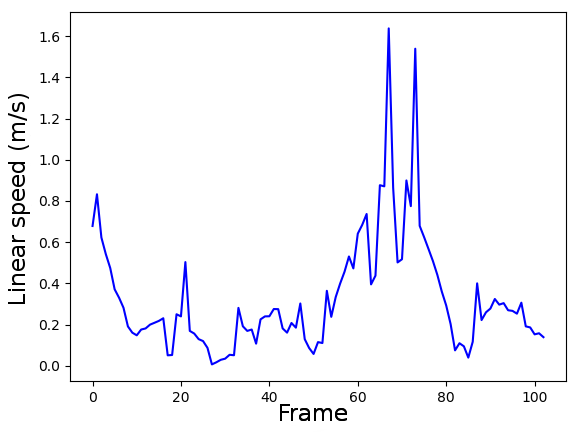
\includegraphics[scale=0.7]{img/linear_speed_artifacts.png}
	\end{frame}
	
	\begin{frame}{Incohérence des positions successives}
	Plusieurs hypothèses :
		\begin{center}
				\begin{table}[h!]
				\resizebox{\linewidth}{!}{%
				\begin{tabular}{l|l|l}
					& \makecell{Interpolation} & Pas d'interpolation \\\hline
					\makecell{Intervalle de temps\\constant} & \makecell{Mauvaise interpolation} & \textit{Frames} manquantes                  \\\hline
					\makecell{Intervalle de temps\\non-constant} & \makecell{Mauvaise posture\\dû a un indice temporel erroné} & \makecell{\textit{Frames} affichées\\au mauvais moment}
				\end{tabular}}
				\end{table}
		\end{center}
	\end{frame}
	
	\begin{frame}{Filtrage des vitesses}
		\begin{itemize}[label=$\bullet$]
			\item Travail sur les descripteurs extraits et non les valeurs de position et d'orientation
			\item Filtre de Savitsky-Golay : régression sur une fenêtre glissante cherchant à minimiser l'erreur au sens des moindres carrés pour un point donné 
			\item Paramètres : taille de la fenêtre, degré du polynôme	
			\item Détermination empirique de la taille de la fenêtre : $\frac{\texttt{frames}}{4}$ 	
		\end{itemize}
	\end{frame}
	
	\begin{frame}{Effet de la taille de la fenêtre}
	\centering
		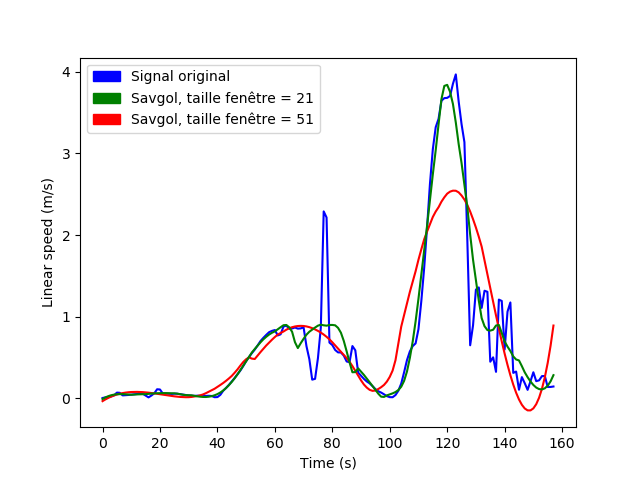
\includegraphics[scale=0.6]{img/savgol_comparison_all_3_at_once.png}
	
	\end{frame}
	
	\begin{frame}{Résultat du filtrage}
	\centering
		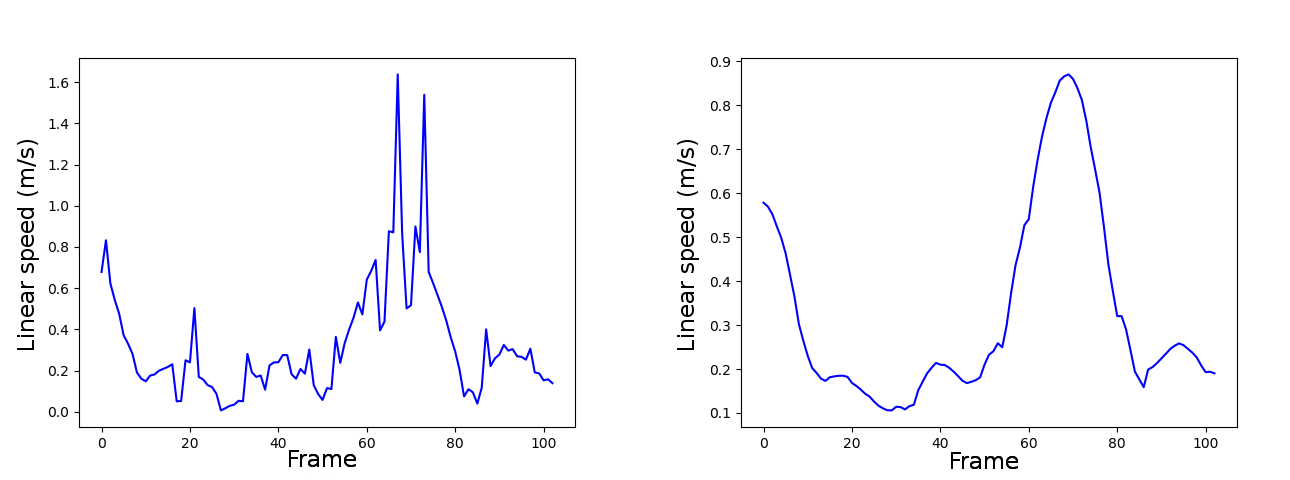
\includegraphics[scale=0.4]{img/before_after_savgol.png}
	\end{frame}
	
	\begin{frame}{Extraction du moment d'intérêt}
	\centering
		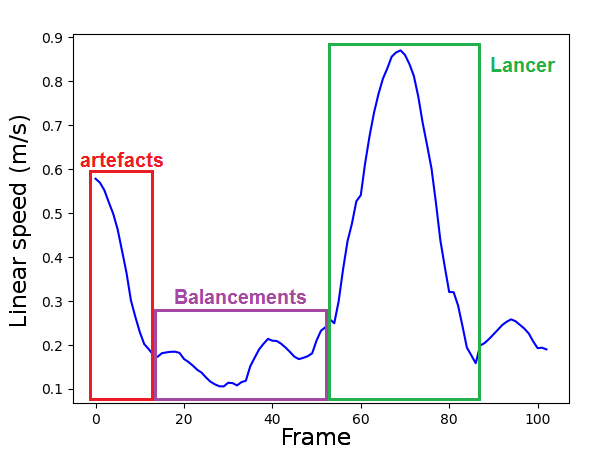
\includegraphics[scale=0.4]{img/after_savgol_explained.png}
	\end{frame}
	
	\section{Extraction du moment d'intérêt}
	\begin{frame}{\secname}
	\centering
		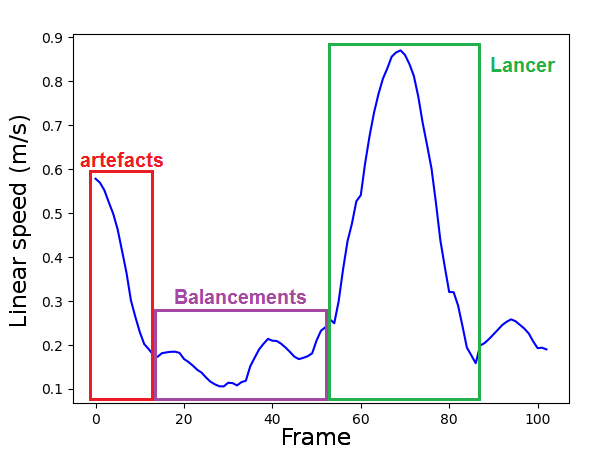
\includegraphics[scale=0.4]{img/after_savgol_explained.png}
	\end{frame}
	
	\section{Aide à l'expert}
	\begin{frame}{\secname}
	Objectif : assister l'expert dans sa tâche d'évaluation du geste, en lui permettant d'obtenir un retour visuel sur les différences entre le geste de l'apprenant et le sien.
	Pré-requis :
	\begin{itemize}[label=$\bullet$]
		\item Données de l'expert réparties en bons gestes / gestes correspondant à un défaut
		\item Données de l'apprenant
		\item Liste de descripteurs à associer aux défauts
	\end{itemize}
	\end{frame}
	
	\begin{frame}{Déroulement}
	\begin{itemize}
		\item \textbf{1.} (Facultatif) Normalisation des données
		\item \textbf{2.} Clustering des données de l'expert, afin d'obtenir deux groupes correspondant aux bons et aux mauvais gestes
		\item \textbf{3.} Comparaison des données de l'apprenant à celles de l'expert
		\item \textbf{4.} Retour sous forme visuelle
	\end{itemize}
	
	\end{frame}
	
	\begin{frame}{Étape de clustering}
	\centering
		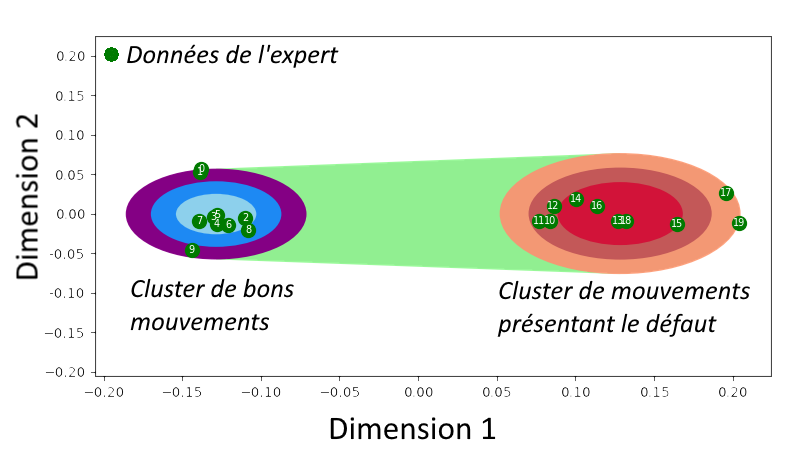
\includegraphics[scale=0.5]{img/feedback_expert_cluster_example.png}
	\end{frame}
	
	\begin{frame}{Étape de comparaison}
	\centering
		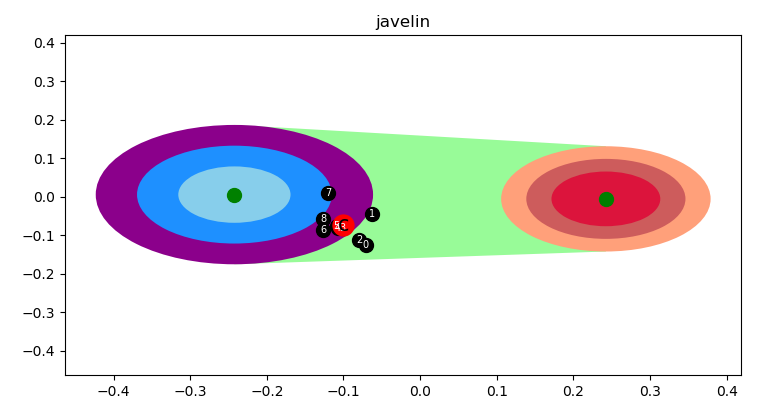
\includegraphics[scale=0.4]{img/feedback_one.png}
	\end{frame}
	
	\begin{frame}{Retour donné à l'expert}
	\centering
		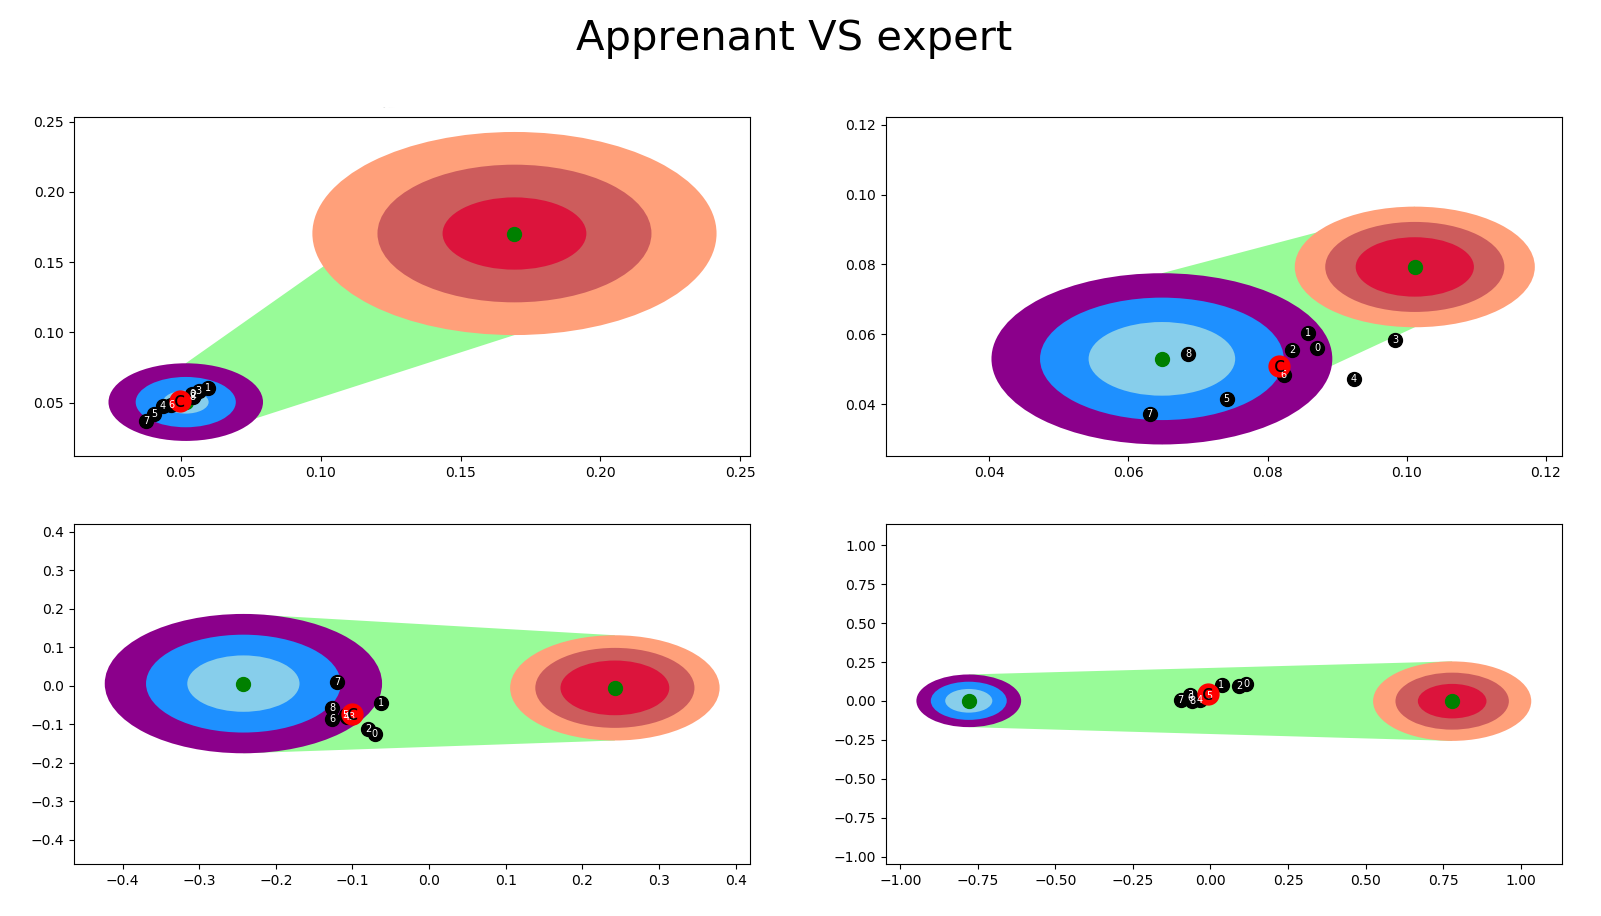
\includegraphics[scale=0.25]{img/feedback_grp_example.png}
	\end{frame}

	\part{Expérimentations}
	\section{Hypothèses de recherche}
	\begin{frame}{\secname}
		\begin{itemize}[label=$-$]
			\item \textbf{H1} : Il est possible de regrouper les gestes selon leurs propriétés cinématiques communes.
			\item \textbf{H2} : Il est possible de séparer les gestes des apprenants en deux groupes correspondant à une dichotomie geste réussi / geste raté afin de déterminer, pour une situation d'apprentissage donnée, les propriétés d'un ensemble fini de gestes réussis.
			\item \textbf{H3} : Il est possible de séparer les gestes en fonction de propriétés attendues et identifiées au préalable par l'expert.
		\end{itemize}
	\end{frame}
	
	\begin{frame}
		\begin{itemize}[label=$-$]
			\item \textbf{H4} : Il est possible de corriger chaque défaut du geste de l'apprenant, en lui indiquant les défauts majeurs à corriger en premier. Un défaut majeur est identifié par la plus grande distance séparant le mouvement courant de l'apprenant, du groupe de gestes acceptables ayant éliminé ce défaut.
			\item \textbf{H5} : L'utilisation du système MLA basée sur l'hypothèse 4 permet d'améliorer l'apprentissage du geste par rapport à une situation sans le système MLA.
			\item \textbf{H6} : L'utilisation du système MLA en tant qu'assistant à l'enseignant permet d'améliorer l'apprentissage du geste par rapport à une situation sans MLA, et à une situation avec MLA et sans enseignant.
		\end{itemize}
	\end{frame}

	\section{Protocole commun}
	\begin{frame}{Protocole commun aux trois expérimentations}
		\begin{itemize}[label=$\bullet$]
			\item Instructions données à l'apprenant
			\item Mesure selon les préconisations de NOITOM
			\item Calibrations de la combinaison d'acquisition de mouvement
			\item familiarisation avec la combinaison 
		\end{itemize}
	
		\centering
		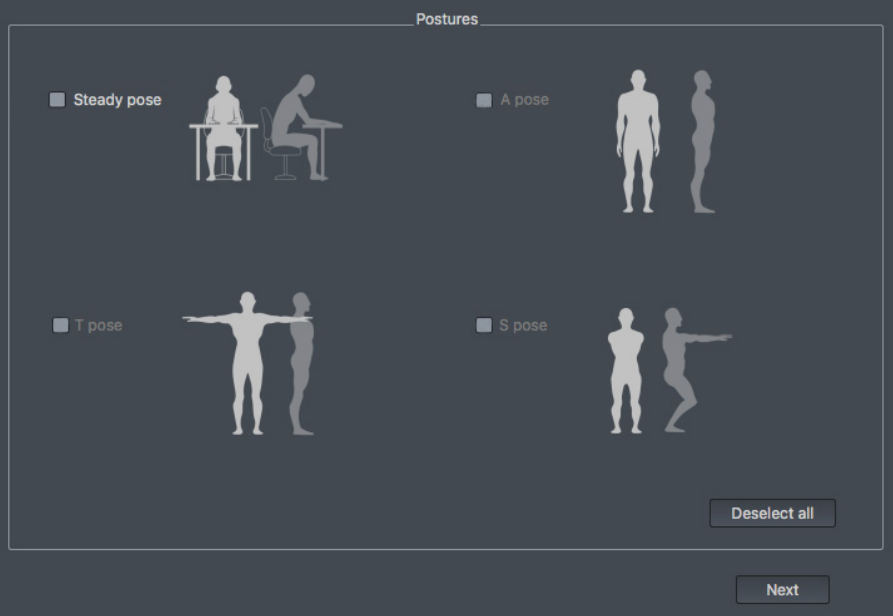
\includegraphics[scale=0.3]{img/percpetion_neuron_calibrations.png}
	\end{frame}
	
	\section{Métriques calculées}
	\begin{frame}{\secname : Average Silhouette Score (\textit{ASS})}
		\begin{block}{Silhouette Score}
			Calcule la bonne appartenance d'un point au cluster qui lui est assigné, en calculant la distance de ce point à tous les autres contenus dans le même cluster par rapport à ceux des autres clusters.
		\end{block}
		
		\begin{block}{Average Silhouette Score \mycite{Rousseeuw1987Sag}}
			Moyenne des Silhouette Score de chaque point de donnée.
		\end{block}
	\end{frame}
	
	\begin{frame}{Average Silhouette Score (\textit{ASS})}
		\begin{itemize}[label=$\bullet$]
			\item $[0;0.25]$ : aucune structure n’est discernable au sein des données
			\item$ ]0.25; 0.5]$ : il existe une structure, bien que mal définie, voire artificielle
			\item $]0.5;0.70
			]$ : une structure existe au sein des données (séparation correcte des clusters)
			\item $]0.7;1]$ : une structure est clairement définie au sein des données (très bonne séparation des clusters)
		\end{itemize}
	\end{frame}
	
	\begin{frame}{\secname : Adjusted Rand Index (\textit{ARI})}
		\begin{block}{Adujsted Rand Index \mycite{Morey1984ARI}}
			Mesure de similarité entre deux partitionnements de données différents. Cette mesure est un ajustement du Rand Index \mycite{Rand2971RI}. Une valeur de 1 indique une correspondance parfaite entre les deux partitionnement, alors qu'une valeur de 0 indique une affectation aléatoire des données. La normalisation induite par l'ajustement peut produire des valeurs négatives \mycite{Meila2007Cca}. 
		\end{block}
	\end{frame}

	\section{Lancer de balle}
	\subsection{Objectifs et principe}
	\begin{frame}{\secname : \subsecname}
		\begin{block}{Objectif}
			Vérifier si le système est capable de séparer les gestes selon un étiquetage vérifiable par un humain à l'aide des descripteurs et des algorithmes choisis (\textbf{H1}, \textbf{H2}).
		\end{block}
	
		\begin{block}{Principe}
			Lancer une balle dans une corbeille parmi deux disposées devant les participants en ligne : l'une est située à 2 mètres devant la personne, et l'autre est située à 3.5 mètres devant la personne
		\end{block}
		
	\end{frame}
	
	\subsection{Schéma de l'installation}
	\begin{frame}{\subsecname : \subsecname}
		\centering
		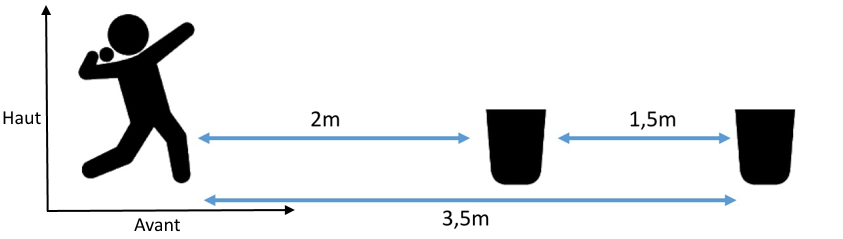
\includegraphics[scale=0.5]{img/ball_throwing.png}
	\end{frame}
	
	\subsection{Étiquetage des données et participants}
	\begin{frame}{\subsecname : \subsecname}
		\begin{block}{Étiquetage des données}
			\begin{itemize}
				\item \textbf{1.} le degré de réussite (balle dans la corbeille ou non)
 				\item \textbf{2.} la corbeille visée
				\item \textbf{3.} le type de lancer (lancer par le haut ou par le bas)
			\end{itemize}
		\end{block}
	
		\begin{block}{Participants}
			\begin{itemize}[label=$\bullet$]
				\item 2 participants
				\item 100 lancers par personne
			\end{itemize}
		\end{block}
	\end{frame}
	
	\subsection{Données utilisées}
	\begin{frame}{\secname : \subsecname}
		\begin{block}{Descripteurs}
			\begin{itemize}
				\item la norme du vecteur vitesse (SN)
				\item la norme du vecteur vitesse en X, Y, Z (S x/y/z)
				\item la direction du vecteur vitesse en X, Y, Z (Sd x/y/z)
				\item la norme du vecteur vitesse ainsi que la direction de ce vecteur en X, Y, Z (SNDxyz)
			\end{itemize}
		\end{block}
		
		\begin{block}{Articulations}
			\begin{itemize}
				\item la main
				\item l'avant-bras
				\item le bras
				\item l'épaule
			\end{itemize}
		\end{block}
	\end{frame}
	
	\subsection{Résultats}
	\begin{frame}{\secname : \subsecname}
	Algorithme utilisé : k-means, avec $k=2$.
	\begin{itemize}
		\item Séparation correcte des clusters avec la norme du vecteur vitesse, ainsi que les vecteurs vitesses en x, y et z ($ASS \approx 0.6$) / \textbf{H1} validée dans le contexte de cette expérimentation
		\item Séparation correspondant à l'étiquetage « type de lancer » ($ARI \approx 0.85$)
		\item Séparation ne correspondant pas au degré de réussite du geste : \textbf{H2} non validée
	\end{itemize}
		
	\end{frame}


	\section{Bottle Flip Challenge}
	\subsection{Objectifs et principe}
	\begin{frame}{\secname : \subsecname}
		\begin{block}{Objectif}
			 Déterminer s'il est possible d'obtenir une séparation des données en deux clusters, correspondant au degré de réussite du geste. ( \textbf{H2}).
		\end{block}
	
		\begin{block}{Principe}
			Lancer une bouteille, partiellement remplie, en lui faisant réaliser un salto arrière, avant de retomber parfaitement droite sur la surface désignée.
		\end{block}
		
	\end{frame}
	
	\subsection{Principe illustré}
	\begin{frame}{\secname : \subsecname}
		\centering
		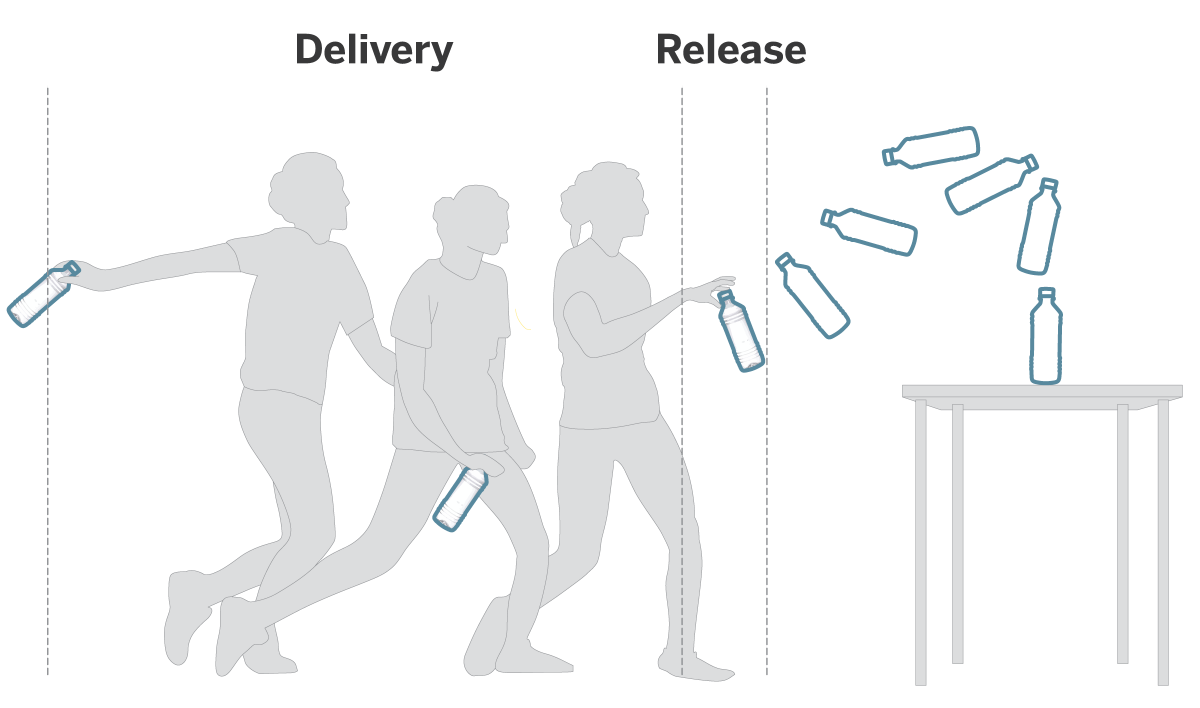
\includegraphics[scale=0.2]{img/BFC_example.png}
	\end{frame}

	\subsection{Schéma de l'installation}
	\begin{frame}{\secname : \subsecname}
		\centering
		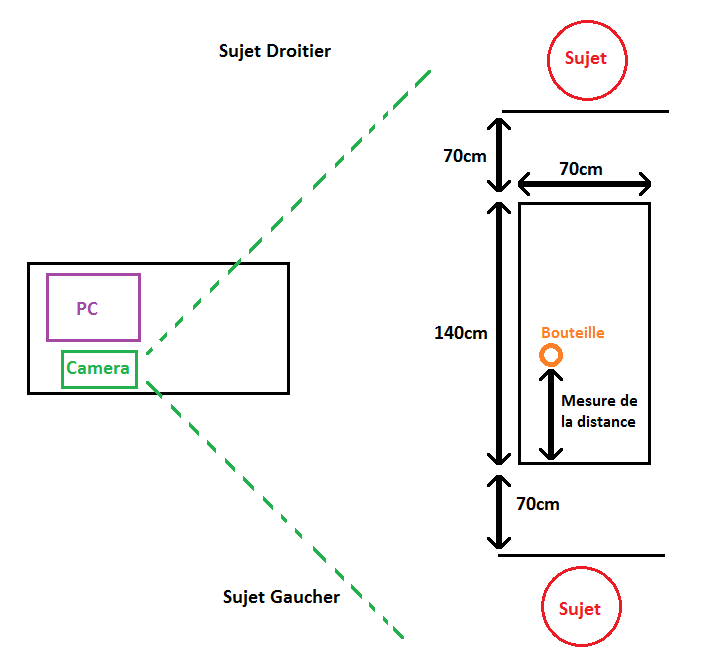
\includegraphics[scale=0.5]{img/BFC_diagram.png}
	\end{frame}
	
	\subsection{Étiquetage des données et participants}
	\begin{frame}{\secname : \subsecname}
		\begin{block}{Étiquetage des données}
			\begin{itemize}
				\item \textbf{1.} le degré de réussite (bouteille retombée correctement ou non)
			\end{itemize}
		\end{block}
	
		\begin{block}{Participants}
			\begin{itemize}[label=$\bullet$]
				\item 13 participants (2 gauchers, 11 droitiers)
				\item 100 lancers par personne
			\end{itemize}
		\end{block}
	\end{frame}
	
	\subsection{Données utilisées}	
	\begin{frame}{\secname : \subsecname}
		\begin{block}{Descripteurs}
			\begin{itemize}
				\item la norme du vecteur vitesse (SN)
				\item la norme du vecteur vitesse en X, Y, Z (S x/y/z)
				\item la direction du vecteur vitesse en X, Y, Z (Sd x/y/z)
				\item la norme du vecteur vitesse ainsi que la direction de ce vecteur en X, Y, Z (SNDxyz)
			\end{itemize}
		\end{block}
		
		\begin{block}{Articulations}
			\begin{itemize}
				\item la main
				\item l'avant-bras
				\item le bras
				\item l'épaule
			\end{itemize}
		\end{block}
	\end{frame}
	
	\subsection{Résultats}
	\begin{frame}{\secname : \subsecname}
	Algorithme utilisé : k-means, avec $k=2$.
	\begin{itemize}
		\item Séparation correcte des clusters pour les vecteurs vitesse en x, y et z des droitiers ($ASS \approx 0.75$) /
		\item Séparation ne correspondant pas au degré de réussite du geste : \textbf{H2} non validée
	\end{itemize}
		
	\end{frame}

	\section{Lancer de fléchettes}
	\subsection{Objectifs et principe}
	\begin{frame}{\secname : \subsecname}
		\begin{block}{Objectifs}
			\begin{itemize}[label=$\bullet$]
				\item Montrer qu'il est possible, à l'aide du système de retours à l'apprenant basé sur les démonstrations de l'expert et l'estimation de valeurs d'acceptabilité empiriques des propriétés du geste, de donner des conseils pertinents lors de la réalisation de ces derniers (\textbf{H3}, \textbf{H4})
			 	\item Montrer qu'une amélioration du geste, en termes de précision du tir et de la « forme » du mouvement résultait de ces conseils (\textbf{H5})
			 	\item Évaluation en terme d'usage de l'efficacité du système selon les modalités précédemment citées : utilisation du système seul, ou utilisation conjointe avec l'analyse de l'expert (\textbf{H6})
			 \end{itemize}
		\end{block}
	
		\begin{block}{Principe}
			Lancer de fléchettes (sport)
		\end{block}
		
	\end{frame}
	
	\subsection{Position de tir}
	\begin{frame}{\secname : \subsecname}
		\centering
		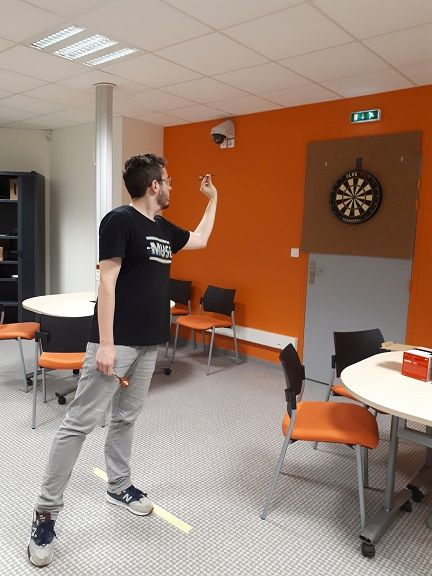
\includegraphics[scale=0.3]{img/darts_position_alt.jpg}
	\end{frame}

	\subsection{Schéma de l'installation}
	\begin{frame}{\secname : \subsecname}
		\centering
		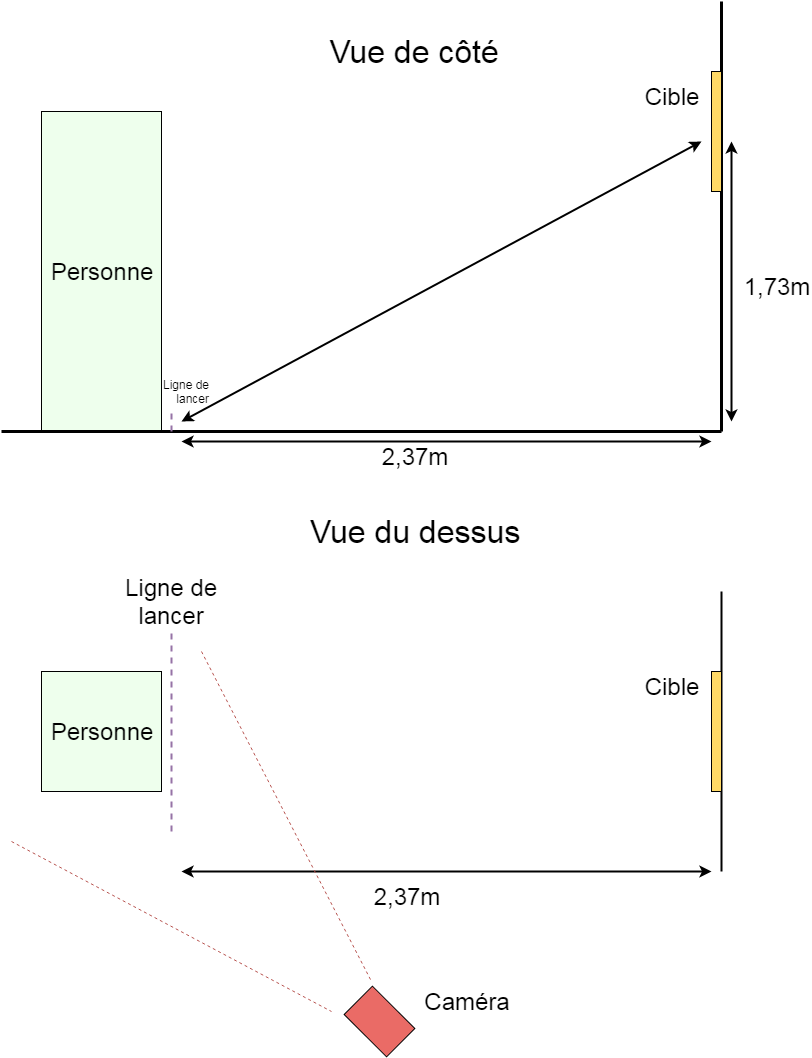
\includegraphics[scale=0.2]{img/Darts_scheme.png}
	\end{frame}
	
	\subsection{Acquisition des données de l'expert et participants}
	\begin{frame}{\secname : \subsecname}
		\begin{block}{Acquisition des données de l'expert}
			\begin{itemize}
				\item \textbf{1.} Identification des défauts quantifiables
				\item \textbf{2.} Capture de mouvements de lancers corrects réalisés par l'expert
				\item \textbf{3.} Pour chaque défaut, capture de mouvements de lancers par l'expert présentant ce défaut 
			\end{itemize}
		\end{block}
	
		\begin{block}{Participants}
			\begin{itemize}[label=$\bullet$]
				\item 45 participants, répartis en 3 groupes de 15 personnes :
				\begin{itemize}
					\item \textbf{Groupe 1} : Conseils de l'expert seulement
					\item \textbf{Groupe 2} : Conseils du système seulement
					\item \textbf{Groupe 3} : Expert s'appuyant sur le système pour donner ses conseils
				\end{itemize}
				\item 36 lancers par personne ($4 \times 9$ lancers)
			\end{itemize}
		\end{block}
	\end{frame}
	
	\subsection{Défauts}
	\begin{frame}{\subsecname : leaning}
		Défaut : corps qui se penche en avant lors du lancer (\textit{leaning})\\
		\centering
		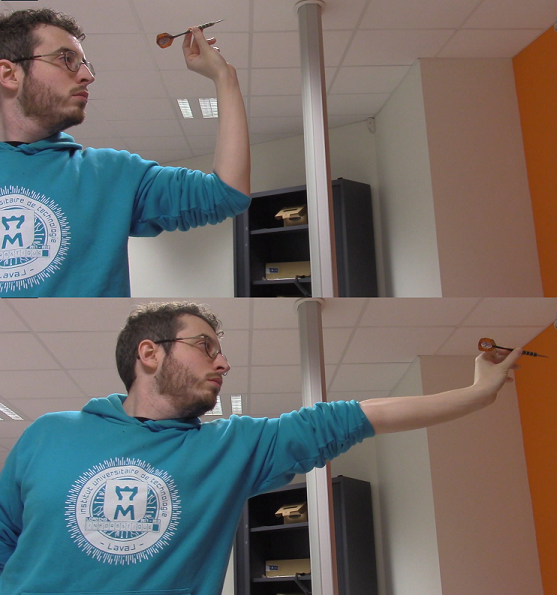
\includegraphics[scale=0.4]{img/darts_leaning_final.png}
	\end{frame}

	\begin{frame}{\subsecname : Elbow move}
		Défaut : coude qui bouge (au lieu de seulement pivoter) lors du lancer (\textit{elbow move})\\
		\centering
		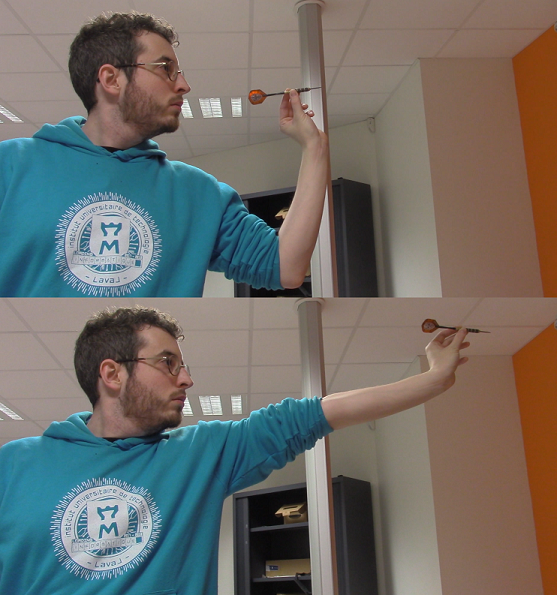
\includegraphics[scale=0.4]{img/darts_elbow_move_final.png}
	\end{frame}

	\begin{frame}{\subsecname : Javelin}
		Défaut : main qui passe à côté ou derrière la tête lors du lancer, appelé « lancer type javelot » (\textit{javelin})\\
		\centering
		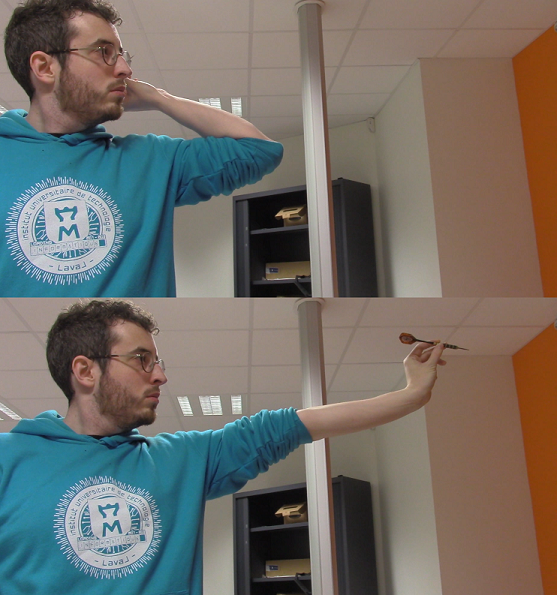
\includegraphics[scale=0.4]{img/darts_javelin_final.png}
	\end{frame}

	\begin{frame}{\subsecname : Align arm}
		Défaut : bras qui part vers la gauche ou vers la droite lors du lancer (\textit{align arm})\\
		\centering
		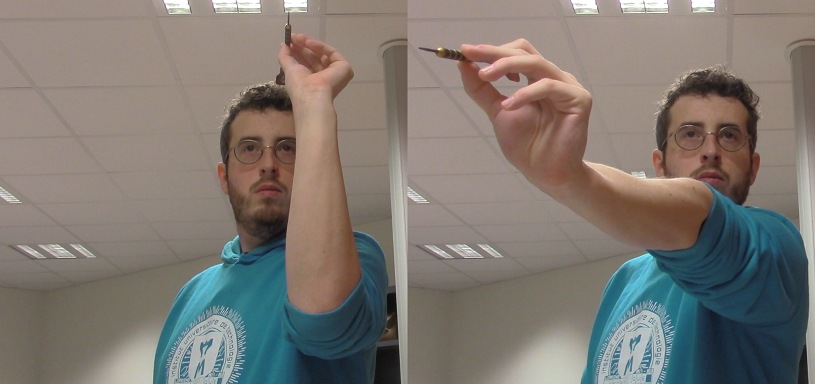
\includegraphics[scale=0.4]{img/darts_align_arm_final.png}
	\end{frame}
	
	\subsection{Données utilisées}
	\begin{frame}{\secname : \subsecname}
		\begin{block}{Descripteurs}
			\begin{itemize}[label=$\bullet$]
				\item Leaning : vitesse moyenne des deux épaules
				\item Elbow move : vitesse moyenne de coude et de l'épaule du côté de la préférence manuelle de la personne
				\item Javelin : distance en x, y et z de la main par rapport à la tête
				\item Align arm : moyenne de la largeur, ainsi que de l'écart-type, de la boîte englobante allant de la main à l'épaule du côté de la préférence manuelle de la personne
			\end{itemize}
		\end{block}
	\end{frame}
	
	\subsection{Déroulement}
	\begin{frame}{\secname : \subsecname}
		\begin{itemize}[label=$\bullet$]
			\item Pré-questionnaire : taille, niveau d'expertise auto-évalué aux fléchettes (échelle de Likert à 7 réponses), ainsi que toute pratique actuelle d'un sport
			\item Début de l'expérimentation
			\item 9 lancers, suivit de deux conseils, 4 fois d'affilé
			\item Post-questionnaire : ressenti de la personne par rapport à la combinaison, à la progression de son geste et à l'auto-évaluation de sa performance
		\end{itemize}
		
	\end{frame}
	
	\subsection{Résultats}
	\begin{frame}{\secname : \subsecname}
	Algorithme utilisé : k-means, avec $k=2$.
	
	\begin{table}[h]
		\centering
		\begin{tabular}{c|c|c}
			& Silhouette Score & Adjusted Rand Index\\\hline
			Leaning & 0.85 & 1\\
			Elbow move & 0.58 & 0.47\\
			Javelin & 0.79 & 1\\
			Align arm & 0.53 & 1\\
		\end{tabular}
	\end{table}
		
		Hypothèse \textbf{H3} validée dans le contexte de cette expérimentation
		
	\end{frame}
	
	\begin{frame}{\secname : \subsecname}
		\begin{block}{Évaluation}
			Deux approches, en intergroupe et en intragroupe :
			\begin{itemize}[label=$\bullet$]
				\item Amélioration de l'objectif du mouvement (distance par rapport au centre de la cible)
				\item Amélioration des propriétés du mouvement (rapprochement du centroïde des données de l'apprenant au bon cluster de l'expert)
			\end{itemize}
		\end{block}
	\end{frame}
	
	\begin{frame}{\secname : \subsecname}
		En premier lieu, test de normalité : Shapiro-Wilk et d'Agostino-Pearson
		\begin{table}[]
			\begin{adjustbox}{max width=\textwidth}
			\begin{tabular}{l|l|l}
				Type de distribution & Normale & Non-normale \\\hline
				Intergroupe & ANOVA & Kruskal-Wallis \\
 				& Levene & Wilcoxon-Mann-Whitney \\
 				& Student paire-à-paire &  \\\hline
				Intragroupe & Student sur deux échantillons & Rangs signés de Wilcoxon
			\end{tabular}
			\end{adjustbox}
		\end{table}
	\end{frame}
	
	\begin{frame}{\secname : \subsecname}
		Amélioration significatives en intragroupe entre les jeu 1 et 4 : \textit{leaning} et \textit{elbow move} pour tous les groupes, \textit{javelin} et \textit{align arm} pour le groupe 2 : \textbf{H4} est validée pour le groupe 2, et partiellement validée pour les autres groupes\\
		\vspace{1cm}
		Pas d'amélioration significatives en intergroupe : \textbf{H5} et \textbf{H6} ne sont pas validées
		
	\end{frame}
	
	\subsection{Limites}
	\begin{frame}{\secname : \subsecname}
		\begin{itemize}[label=$\bullet$]
			\item Phénomène d'auto-correction de l'expert
			\item Nombre de lancers pour les apprenants faibles (36)
			\item Pause entre chaque série de 9 lancers : perte du geste
			\item Systématiquement 2 conseils donnés
			\item Analyse de l'expert seul plus difficile dans le cadre de l'expérimentation
			\item Dans une situation d'apprentissage réelle, données extérieures au mouvement de l'apprenant
			\item L'évaluation du système suppose une prise en compte des conseils donnés
		\end{itemize}
	\end{frame}
	
	\part{Synthèse des contributions et perspectives}
	\section{Synthèse des contributions}
	
	\begin{frame}{\secname}
		\begin{itemize}[label=$\bullet$]
			\item Proposition d'un EIAH dédié à l'apprentissage des gestes
			\item Permet le pré-traitement des données, l'extraction de descripteurs et l'analyse du mouvement de l'apprenant
			\item Généricité pensée dès la conception
			\item Expérimentations menées pour valider les différents aspects du système
		\end{itemize}
	\end{frame}
	
	\section{Limites des travaux présentés}
	\begin{frame}{\secname}
		\begin{itemize}[label=$\bullet$]
			\item Manque d'interface graphique pour utiliser le système
			\item Pertinence des indicateurs visuels à analyser
			\item L'utilisation du Perception Neuron pour la captation implique l'utilisation de techniques de filtrage pour les données
			\item Dans le cadre de l'expérimentation du lancer de fléchettes, faible nombre de lancers
		\end{itemize}
	\end{frame}
	
	\section{Perspectives}
	\begin{frame}{\secname}
		\begin{itemize}[label=$\bullet$]
			\item Explication des données non-alignées
			\item Création de nouveaux descripteurs à l'aide d'un système fondé sur des patrons de conception
			\item Expérimentation à plus grande échelle
			\item Expérimentation dans d'autres domaines applicatifs
			\item Expérimentation d'apprentissage en autonomie
			\item Clustering récursif
		\end{itemize}
	\end{frame}


\end{document}

\iffalse

\if







